\chapter{Negocio}

\section{Introducción}

Esta capa se refiere a los procesos de negocio, servicios, funciones y eventos ce cada una de las unidades de negocio. Esta capa ofrece productos y servicios a clientes externos, que se realizan en la organización mediante procesos de negocio realizados por actores y roles empresariales.

\begin{figure}[th!]
	\centering
	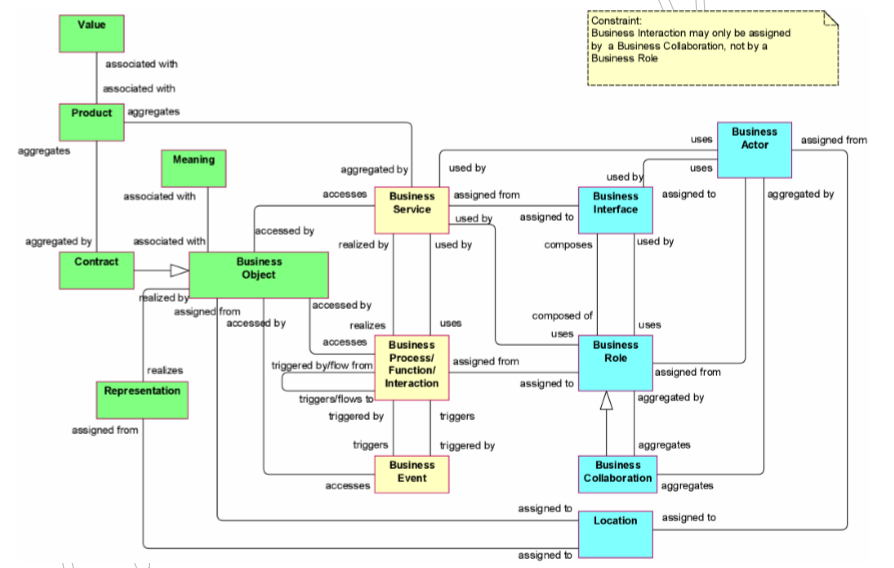
\includegraphics[width=0.6\linewidth]{arquitectura/imagenes/negocio}
	\caption{Metamodelo de la capa de negocio }
	\label{fig:negocio}
\end{figure}

La capa de negocio contiene la lógica principal de procesamiento de datos dentro de nuestra aplicación Web. Se comunica con la capa de presentación para obtener las entradas del usuario y presentar la información resultante, así como la capa de acceso a datos o directamente con servicios para realizar sus operaciones.

\newpage

\section{Punto de Vista de Organización}

\subsection{Modelo}
\begin{figure}[th!]
	\centering
	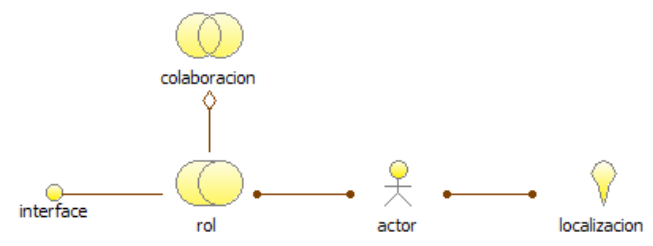
\includegraphics[width=0.5\linewidth]{arquitectura/imagenes/modeloOrganizacion}
	\caption{Metamodelo de Punto de Vista de Organización  \cite{pun1}}
	\label{fig:metamodelo de punto de vista de organizacion}
\end{figure}
El punto de vista de la organización se centra en la organización (interna) de una empresa, un departamento, una red de empresas o de otra entidad organizativa. Es posible presentar modelos en este punto de vista como diagramas de bloques anidados, pero también de una manera más tradicional, como los organigramas. El punto de vista de la Organización es muy útil  en la identificación de competencias, autoridad y responsabilidades en una organización.


\subsection{Caso de estudio}


\begin{figure}[!th]
	\centering
	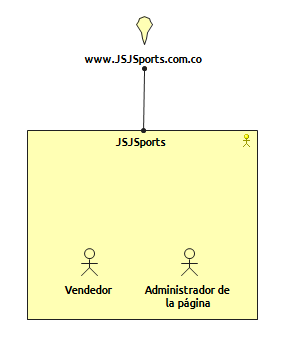
\includegraphics[width=0.5\linewidth]{arquitectura/imagenes/vistaOrganizacion}
	\caption{Punto de Vista de Organización}
	\label{fig:Punto de vista organizacion}
\end{figure}

En la figura 5.3 se puede apreciar que la empresa JSJ sports la cual es un actor tiene un sitio web, localizado en una dirección electrónica, a su vez se observa que se encuentra conformada por un vendedor y un administrador.

\newpage


\section{Punto de Vista de cooperación de Actor}

\subsection{Modelo}
\begin{figure}[th!]
	\centering
	\includegraphics[width=0.5\linewidth]{arquitectura/imagenes/modelocooperacionActor}
	\caption{Metamodelo de Punto de Vista de Cooperación de Actor \cite{pun2}}
	\label{fig:metamodelo de punto de vista de cooperacion de actor}
\end{figure}

El punto de vista de la Cooperación Actor se centra en las relaciones de los actores entre sí y su entorno. Un ejemplo común de esto es el "diagrama de contexto", que pone a una organización en su entorno, que consiste en partes externas, como clientes, proveedores y otros socios comerciales. Es muy útil para determinar las dependencias externas y las colaboraciones y muestra la cadena de valor o la red en la que actúa el actor.


\subsection{Caso de estudio}

\begin{figure}[th!]
	\centering
	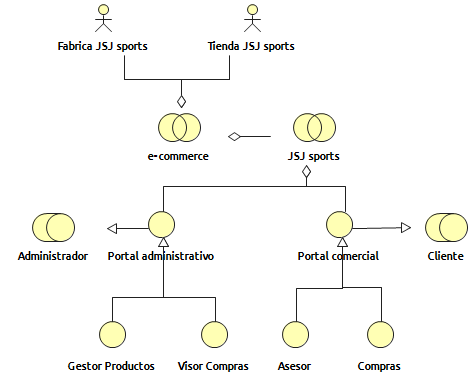
\includegraphics[width=0.6\linewidth]{arquitectura/imagenes/VistaCooperacionActor}
	\caption{Punto de vista Cooperacion Actor}
	\label{fig:Punto de vista Cooperacion Actor}
\end{figure}

En la figura 5.5 se puede observar que la empresa JSJ sports se encuentra conformada por un e-commerce, que tiene como componentes la fabrica y la tienda de la empresa respectivamente, a su vez tendra dos portales, un portal comercial que sera la interfaz de JSJSports para los clientes, el cual tiene una interfaz de asesor y una de compras y un portal administrativo que se compone de dos interfaces, un gestor de productos y un visor de compras y le permitirá al administrador realizar toda la gestión y configuración del sitio.

\newpage

\section{Punto de Vista de Función de Negocio}

\subsection{Modelo}
\begin{figure}[th!]
	\centering
	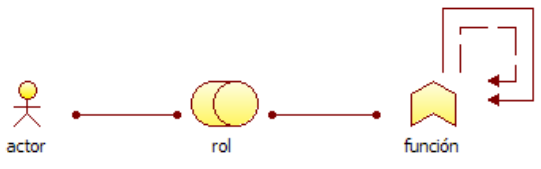
\includegraphics[width=0.5\linewidth]{arquitectura/imagenes/modeloFuncionNegocio}
	\caption{Metamodelo de Punto de Vista de Función de Negocio \cite{pun3}}
	\label{fig:metamodelo de punto de vista de función de negocio}
\end{figure}
El punto de vista Función de negocio muestra las principales funciones de negocio de una organización y sus relaciones en términos de los flujos de información, valor o bienes entre ellos. Las funciones empresariales se utilizan para representar los aspectos más estables de una empresa en términos de las actividades primarias que realiza, independientemente de los cambios organizacionales o desarrollos tecnológicos. Por lo tanto, la arquitectura de la función comercial de las empresas que operan en el mismo mercado a menudo muestran similitudes cercanas.


\subsection{Caso de estudio}

\begin{figure}[th!]
	\centering
	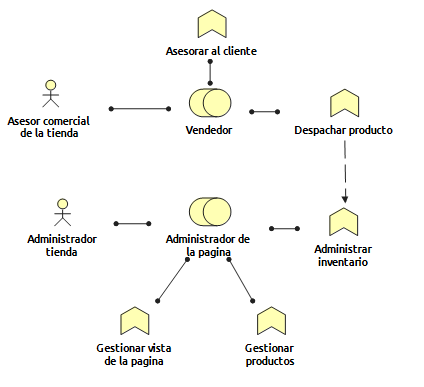
\includegraphics[width=0.6\linewidth]{arquitectura/imagenes/vistaNegocio}
	\caption{Punto de vista de función negocio}
	\label{fig:Punto de vista de funcion de negocio}
\end{figure}

En la figura 5.7 se puede observar como la empresa JSJ sports tiene como principales roles un vendedor y un administrador de la pagina, el primero que se puede especificar como un asesor comercial de la tienda debido a que tiene como funciones asesorar al cliente durante los procesos de compra y despachar el producto una vez este ha sido ordenado, el segundo que se puede especificar como el administrador de la tienda, tiene como funciones gestionar la vista de la pagina, gestionar productos y administrar el inventario que es disparada por la función despachar productos del vendedor. 



\newpage

\section{Punto de Vista de Proceso de negocio}

\subsection{Modelo}
\begin{figure}[th!]
	\centering
	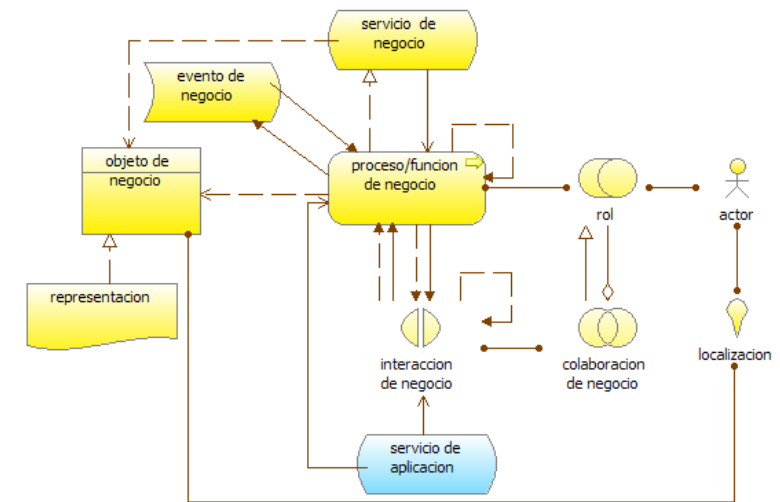
\includegraphics[width=0.6\linewidth]{arquitectura/imagenes/modeloProcesoNegocio}
	\caption{Metamodelo de Punto de Vista de Proceso de Negocio \cite{pun4}}
	\label{fig:metamodelo de punto de vista de proceso de negocio}
\end{figure} 
El punto de vista de Proceso de Negocio se utiliza para mostrar la estructura y composición de alto nivel de uno o más procesos empresariales. 

\subsection{Caso de estudio}

\begin{figure}[th!]
	\centering
	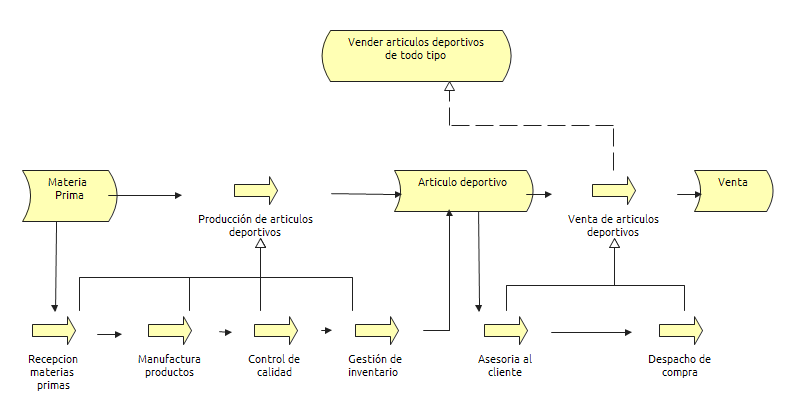
\includegraphics[width=0.6\linewidth]{arquitectura/imagenes/VistaProcesoNegocio}
	\caption{Modelo de Punto de Vista de Proceso de Negocio \cite{pun5}}
	\label{fig:Modelo de punto de vista Proceso de Negocio}
\end{figure}


Como se puede ver en la figura 5.9 el servicio principal de la empresa es el vender artículos deportivos de todo tipo, este servicio depende completamente del proceso venta de artículos deportivos, el cual se divide en los sub-procesos de asesoría al cliente y despacho de la compra. 
\newline
A pesar de que el proceso principal es la venta, se sabe que este depende de otro gran proceso el cual es la producción de los artículos deportivos que se venden, esto es importante puesto que hace parte e los objetivos y misión de la empresa, este proceso a su vez se divide en 4 sub-procesos los cuales son: Recepción de materias primas, manufactura de productos, control de calidad y gestión de inventario.
\newpage

\section{Punto de Vista de Cooperacion Proceso de negocio}

\subsection{Modelo}
\begin{figure}[th!]
	\centering
	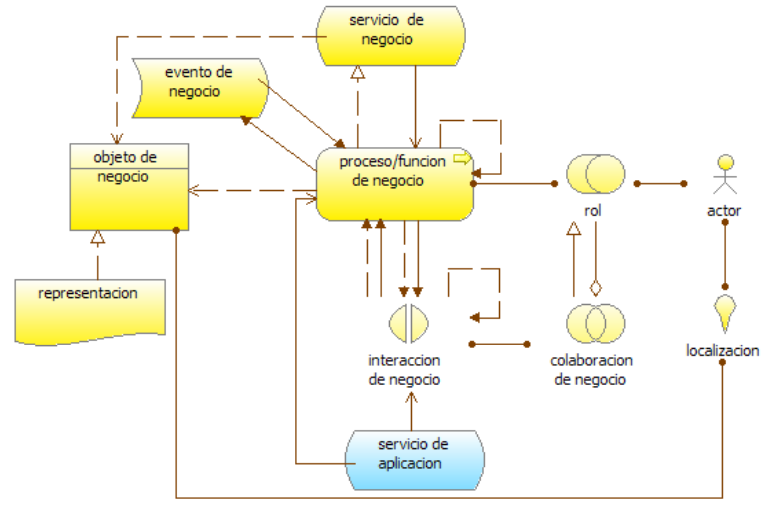
\includegraphics[width=0.6\linewidth]{arquitectura/imagenes/modeloCooperacionProcesoNegocio}
	\caption{Metaodelo de Punto de Vista Cooperación de Proceso de Negocio \cite{pun5}}
	\label{fig:metamodelo de punto de vista de cooperacion proceso de negocio}
\end{figure}
El punto de vista de Cooperación de Proceso de Negocio se utiliza para mostrar las relaciones de uno o más procesos de negocio entre sí y / o con su entorno. Puede utilizarse tanto para crear un diseño de alto nivel de procesos empresariales dentro de su contexto como para proporcionar un gestor operativo responsable de uno o más de dichos procesos con información sobre sus dependencias.

\subsection{Caso de estudio}

\begin{figure}[th!]
	\centering
	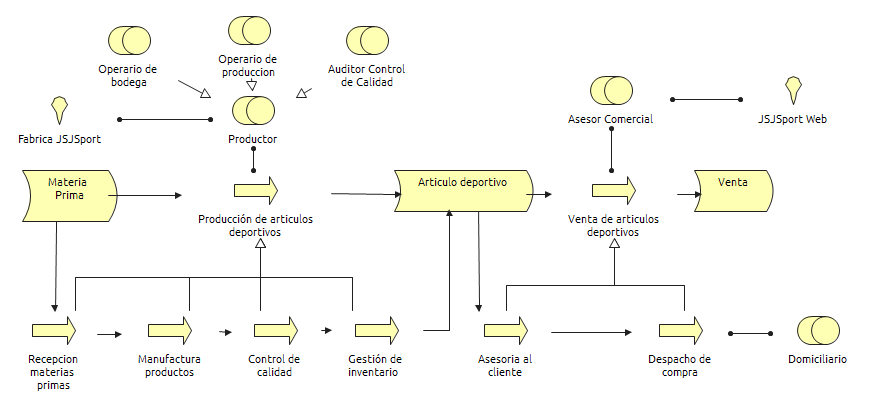
\includegraphics[width=0.6\linewidth]{arquitectura/imagenes/VistaCooperacionProcesoNegocio}
	\caption{Modelo de Punto de Vista Cooperación Proceso de Negocio \cite{pun5}}
	\label{fig:Modelo de punto de vista Cooperacion Proceso de Negocio}
\end{figure}

Al igual que en anterior punto de vista en este modelo se puede ver que la empresa tiene 2 grandes procesos, el primer proceso es el de la producción de artículos deportivos, este proceso es llevado a cabo por el productor en la Fabrica de JSJSport, el rol de productor esta conformado por varios roles, el primero es el operario de bodega quien es el encargado de recibir materias primas y organizar inventarios y productos, el segundo es el operario de producción donde se encuentran todos los encargados de la elaboración del producto y por último el encargado de realizar el proceso de control de calidad.
\newline
El segundo gran proceso es llevado a cabo por el asesor comercial quien asesora al cliente y realiza la venta en la tienda de JSJSport, ademas de esto en el sub-proceso de despacho de compra se incluye el rol de domiciliario quien es el encargado de entregar este producto al cliente.

\newpage

\section{Punto de Vista de Producto}

\subsection{Modelo}
\begin{figure}[th!]
	\centering
	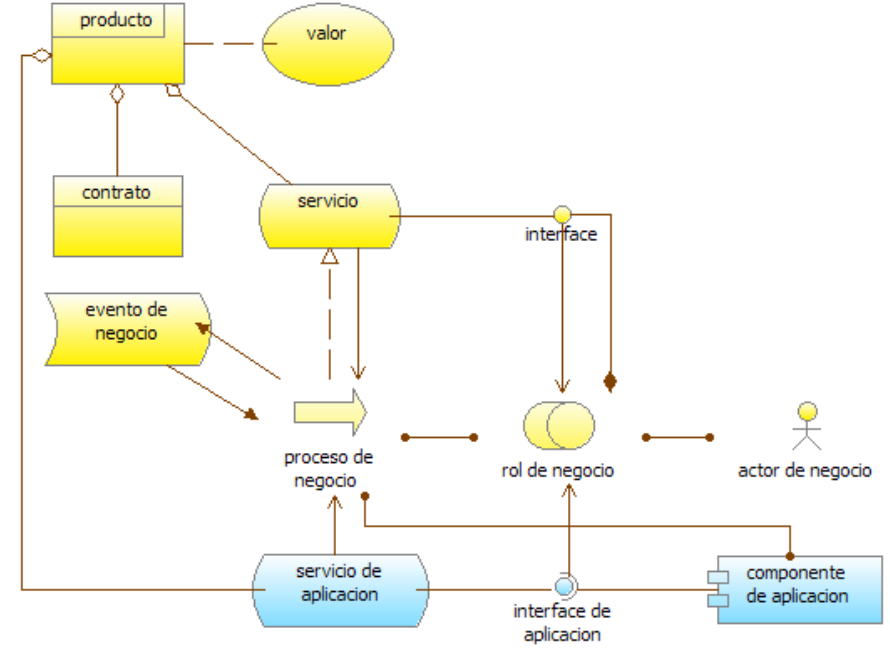
\includegraphics[width=0.5\linewidth]{arquitectura/imagenes/modeloProducto}
	\caption{Metamodelo de Punto de Vista de Producto\cite{pun6}}
	\label{fig:metamodelo de punto de vista de producto}
\end{figure}
El punto de vista del Producto representa el valor que estos productos ofrecen a los clientes u otras partes externas involucradas y muestra la composición de uno o más productos en términos de los servicios constitutivos (comerciales o de aplicación) y los contratos asociados u otros acuerdos.

\subsection{Caso de estudio}

\begin{figure}[th!]
	\centering
	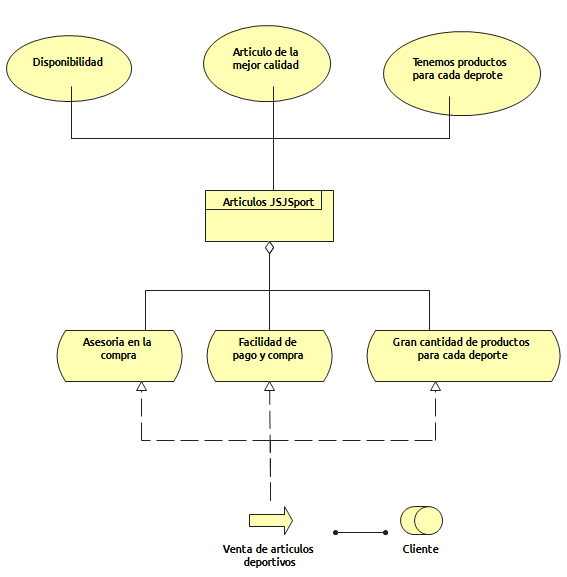
\includegraphics[width=0.5\linewidth]{arquitectura/imagenes/VistaProducto}
	\caption{Modelo de Punto de Vista de Producto \cite{pun5}}
	\label{fig:modelo de punto de vista Producto}
\end{figure}
En la imagen 5.13 se puede observar que el principal servicio de JSJSport es la venta de artículos deportivos al cliente, el producto estrella de la empresa JSJ son los artículos deportivos JSJ, el producto cuenta con 3 diferentes servicios claves para la identidad de la empresa, los cuales son, asesoría al cliente, facilidad de pago y compra, y la gran cantidad de artículos ofrecidos para cada deporte con la cual se busca que en la tienda se tengan los artículos necesarios para cada disciplina deportiva.
A su vez el producto tiene 3 valores, la disponibilidad del producto y de los asesores, la calidad de este producto y la garantía de que el cliente va a encontrar lo que busca.

\newpage

